\documentclass[tikz, border=10pt]{standalone}
\usepackage{pgfplots}
\usepackage{amsmath}
\usetikzlibrary{backgrounds}
\pgfplotsset{compat=1.18}

\begin{document}
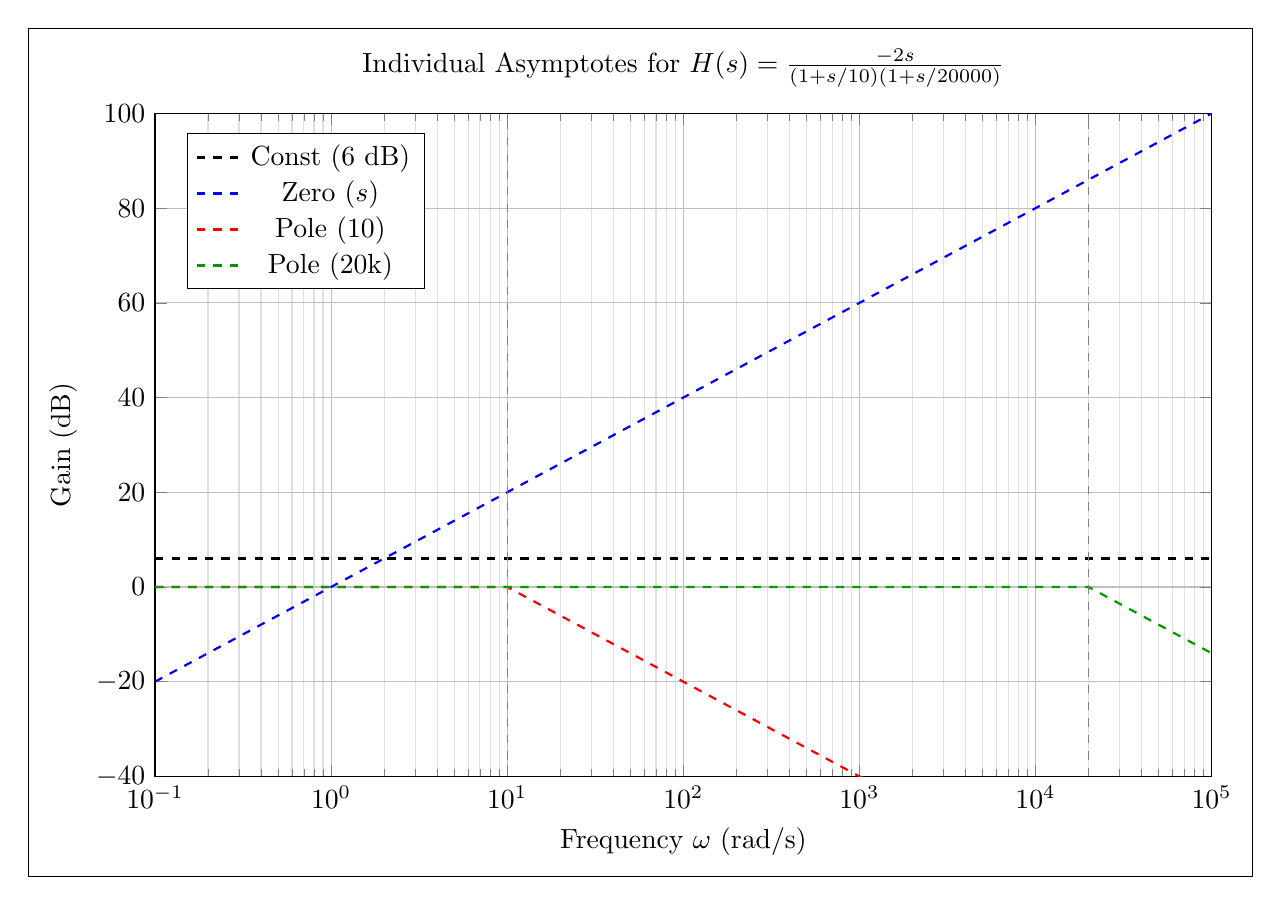
\begin{tikzpicture}[show background rectangle]
    \begin{semilogxaxis}[
        width=15cm, height=10cm,
        title={Individual Asymptotes for $H(s) = \frac{-2s}{(1+s/10)(1+s/20000)}$},
        xlabel={Frequency $\omega$ (rad/s)},
        ylabel={Gain (dB)},
        grid=both,
        xmin=0.1, xmax=100000,
        ymin=-40, ymax=100,
        minor grid style={gray!25},
        major grid style={gray!50},
        legend pos=north west,
    ]

    % 1. Constant K = -2 => 6 dB
    \addplot[black, thick, dashed, domain=0.1:100000] {6};
    \addlegendentry{Const ($6$ dB)}

    % 2. Zero at origin (s) => +20 dB/dec, passing through 0dB at w=1
    \addplot[blue, thick, dashed, domain=0.1:100000] {20*log10(x)};
    \addlegendentry{Zero ($s$)}

    % 3. Pole at 10 => 0 dB until 10, then -20 dB/dec
    % -20*log10(x/10) = -20*(log10(x)-1) = -20log10(x) + 20
    \addplot[red, thick, dashed] coordinates {
        (0.1, 0) (10, 0) (100000, -80)
    };
    \addlegendentry{Pole ($10$)}

    % 4. Pole at 20000 => 0 dB until 20000, then -20 dB/dec
    % -20*log10(x/20000) at 100000 is -20*log10(5) = -13.97
    \addplot[green!60!black, thick, dashed] coordinates {
        (0.1, 0) (20000, 0) (100000, -13.98)
    };
    \addlegendentry{Pole ($20\text{k}$)}

    % Highlight break frequencies
    \draw[dashed, gray] (axis cs:10, -40) -- (axis cs:10, 100);
    \draw[dashed, gray] (axis cs:20000, -40) -- (axis cs:20000, 100);
    
    \end{semilogxaxis}
\end{tikzpicture}
\end{document}
